\subsection{Analysis Object Models}

This subsection depicts FLOps' main components and their relationships in more detail.
The following models are derived from and created to resolve the elicited requirements.
They focus on the user perspective.
It is common to use generalized and abstract UML class diagrams to depict the system's main components, properties, and functions \cite{book:bruegge}.

\begin{figure}[h]
    \centering
    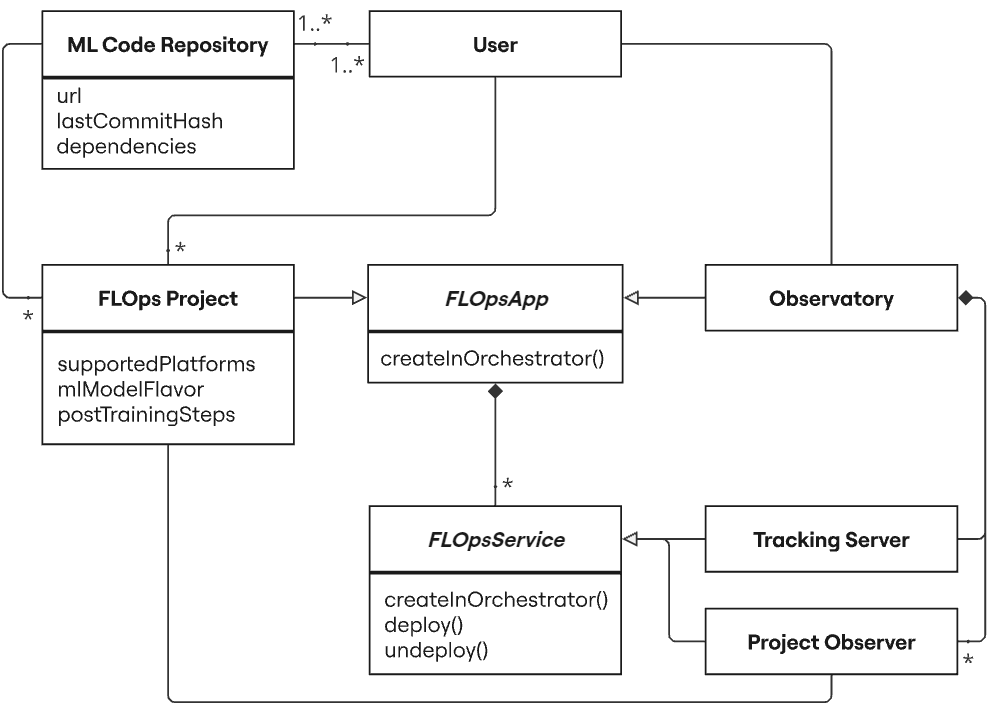
\includegraphics[width=1.0\textwidth]{uml_analysis_object_model_core.png}
    \caption{FLOps Core UML Analysis Object Model}
    \label{fig:uml_core_analysis_object_model}
\end{figure}

Figure \ref{fig:uml_core_analysis_object_model} shows the core FLOps UML analysis object model.
The main workflow is represented and grouped via a FLOps project.
Such a project links all necessary FL and ML/DevOps components to power one FL user request.
A project contains information about the user who requested it, the target platforms that should be supported (e.g., ARM/AMD), and what steps FLOps should perform after training.
If no steps are specified, the FLOps project counts as completed after training.
Available post-training steps include building a containerized image for the trained model and deploying an inference server to serve the trained model.
The ML model flavor indicator tells FLOps what ML framework to expect and work with.
Examples include Keras, Sklearn, or Pytorch.
Each project is associated with exactly one ML code repository.
This repository can be owned by the user or be a public one.
Thus, multiple users can reuse the same repository, and each user can create multiple FLOps projects per repository.
These properties are based on the SLA from the user request.

FLOps uses the concepts of applications and services to manage dependent components and concepts.
Each app can have multiple services.
Services are bound to parent apps and cannot exist on their own.
The orchestrator creates and realizes apps and services as usable components.
Applications themselves are collectors of information and metadata.
They do not run or contain any executable code, images, or similar.
Services are the computational components that can be deployed and un-deployed.
This split is based on Oakestra's applications and services.
The two main FLOps app types are project-based apps and customer-facing ones.

The observatory app is a customer-facing app.
There is exactly one observatory app for each user, whereas users can have multiple projects.
The observatory hosts the tracking server and project observer services.
The tracking server service tracks the projects and individual FL experiments.
It hosts the GUI. 
(It utilizes the MLFlow tracking server mentioned in \ref{subsection:mlflow}.)
When users request/start a new project, the observatory is created with all its components if it does not already exist.
Users can request access to the GUI/tracking server independently from a project.
A project observer service gathers and displays information or updates regarding the project status for the user.
The project observer informs the user of any issues during the project's live time, such as dependency issues during the containerized image builds.
There is one project observer per project to improve readability and comprehension.

\begin{figure}[t]
    \centering
    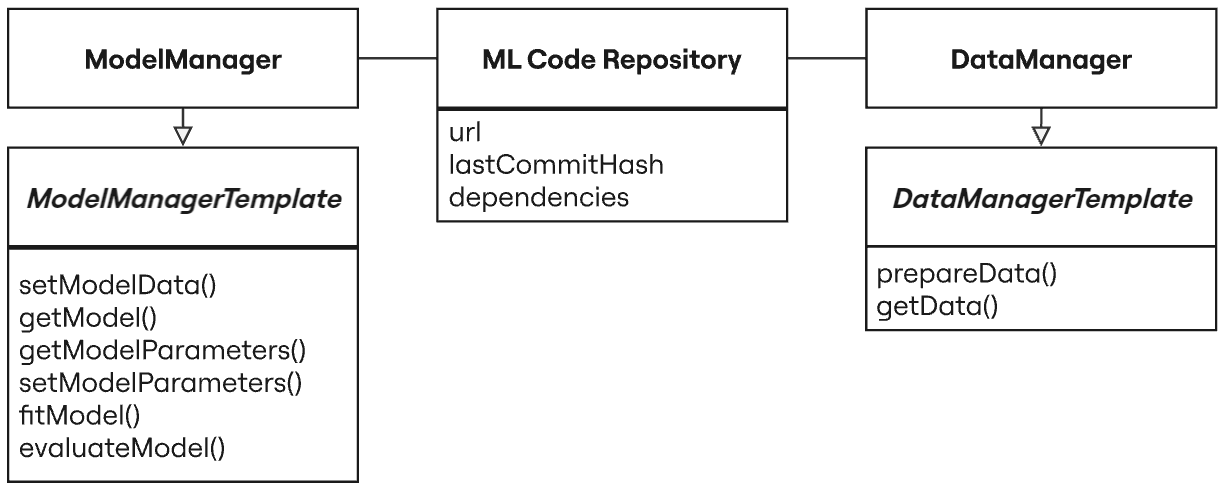
\includegraphics[width=1.0\textwidth]{uml_analysis_object_model_repo.png}
    \caption{FLOps ML Code Repository UML Analysis Object Model}
    \label{fig:uml_repo_analysis_object_model}
\end{figure}

Figure \ref{fig:uml_repo_analysis_object_model} shows additional details of the ML code repositories from the core model.
Users can provide a link to ML code repositories for FLOps to augment and train.
The repository must fulfill the following structural requirements for this to be possible and straightforward.
The repository needs a dedicated file that lists all necessary dependencies to train its model.
Theoretically, it should be possible to extract these requirements dynamically by inspecting the code.
However, this is a complex and error-prone endeavor.
To avoid these issues, users should provide the dependencies they used for training.
\vspace{5mm}
\newline
\textbf{Recommendation}: We recommend running the training locally on some exemplary or mock data and recording the dependencies via MLflow's auto-logging functionality.
This is an easy and viable approach to getting a suitable dependency file.
Note that this does not guarantee compatibility because MLflow's dependency logging can be erroneous.
Before providing the dependency file to FLOps, we recommend ensuring the dependencies are sufficient and compatible.
\vspace{5mm}
\newline
For FLOps to augment and utilize the ML code properly, FLOps requires the repository to implement a model manager and data manager.
The model manager is the interface that accesses the model and its data and parameters.
It further trains and evaluates the model.
It calls its linked data manager to prepare the data and retrieve it once it is ready.
The data itself should not be part of the repository.
The prepare data method will call a FLOps method that will be added during FL augmentation.
The user has to define in \texttt{prepareData} how to pre-process the retrieved data for individual training.
Both managers have an abstract parent class that users can import during implementation for guidelines.
These templates are available as part of the FLOps Utils pip package \cite{flops_utils_pip}.

\begin{figure}[t]
    \centering
    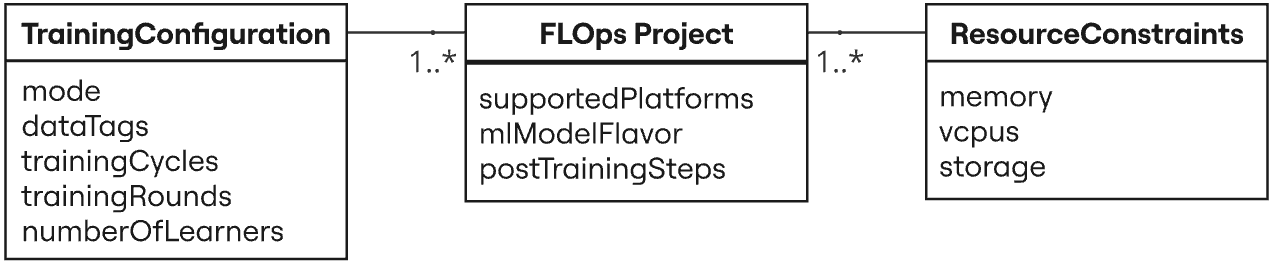
\includegraphics[width=1.0\textwidth]{uml_analysis_object_model_project.png}
    \caption{FLOps Project UML Analysis Object Model}
    \label{fig:uml_project_analysis_object_model}
\end{figure}

Figure \ref{fig:uml_project_analysis_object_model} shows further details about the contents of an FLOps project.
Users can customize their projects via the SLA (\ref{subsection:SLAs}) that is part of their API requests (\ref{subsection:api}).
One possible customization is to specify resource constraints such as memory or storage.
Users can customize the FL training by changing the project's training configuration.
The same ML repository can be trained differently depending on these configurations.
This configuration includes a mode that tells FLOps to perform different types of FL if applicable.
Currently, FLOps supports classic and (clustered) HFL.
The project will only use training data that matches the provided data tags.
The training rounds configure the number of training and evaluation rounds that each learner performs.
Only HFL uses training cycles.
The training rounds mean the number of training rounds performed on each learner per cycle.
A training cycle is the number of training rounds between the root and cluster aggregators, which resemble aggregators and learners in classic FL.
For example, if the user requests three cycles and five rounds, the learners will train five rounds per cycle for three cycles.
Each learner will train for 15 rounds during the entire project runtime.
The depicted attributes are only a subset of currently available and possible configurations.

\begin{figure}[t]
    \begin{adjustwidth}{-0.1\paperwidth}{-0.1\paperwidth}
        \centering
        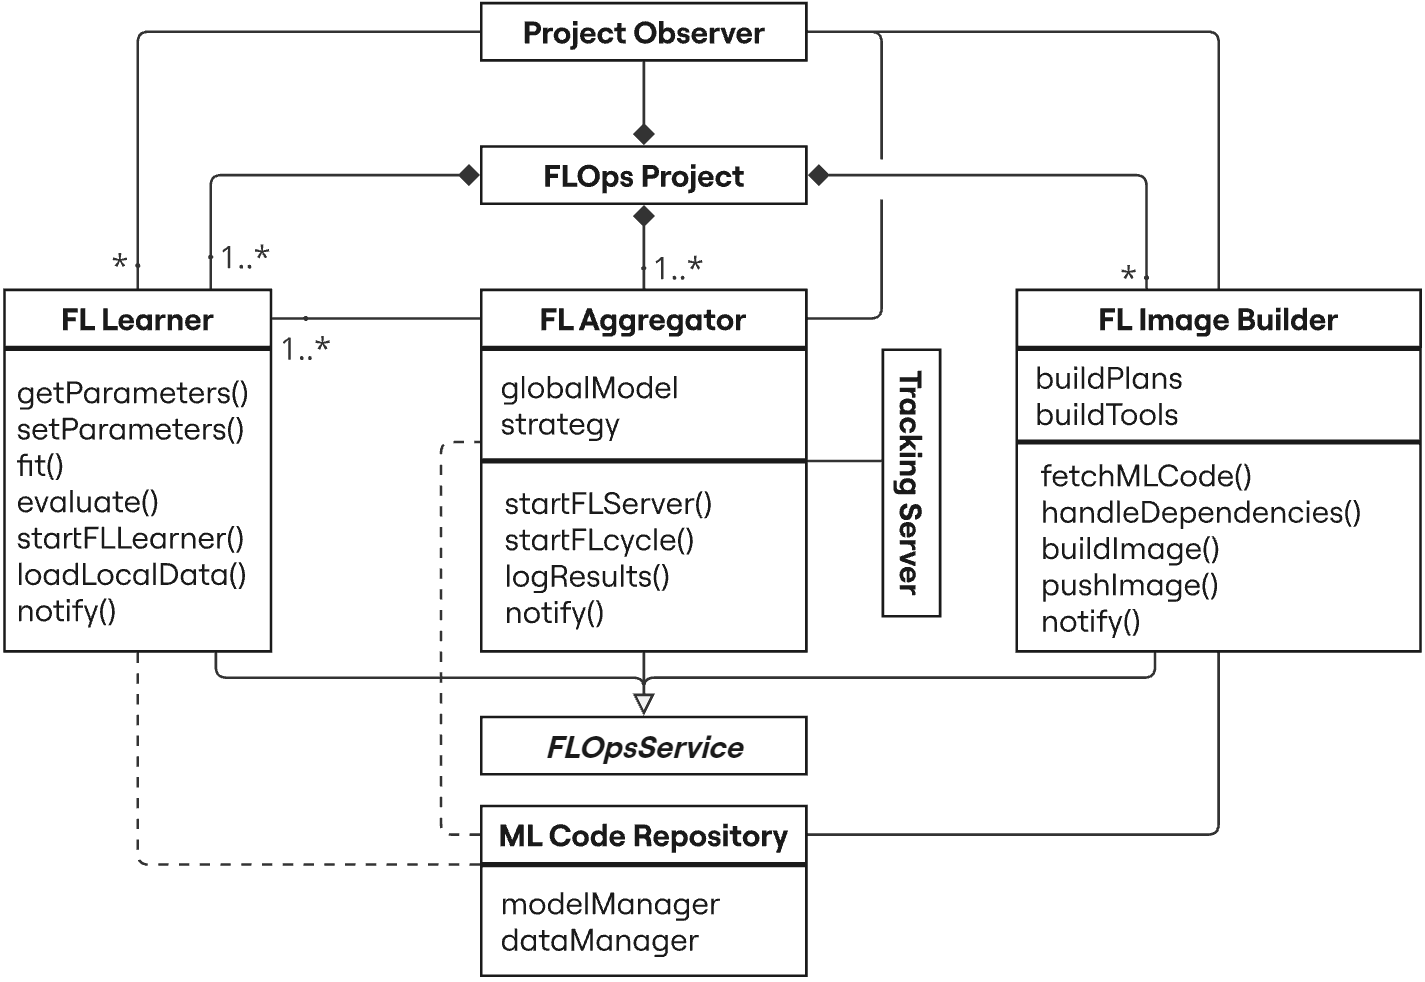
\includegraphics[width=0.80\paperwidth]{uml_analysis_object_model_project_services.png}
        \caption{FLOps Project Services UML Analysis Object Model}
        \label{fig:uml_project_services_analysis_object_model}
    \end{adjustwidth}
\end{figure}

The core figure \ref{fig:uml_core_analysis_object_model} only alluded that a project consists of several services and depicted only the project observer.
Figure \ref{fig:uml_project_services_analysis_object_model} expands upon this and shows important project services and their relationships.
There are three main project services.
The FL image builder is a service that builds containerized images.
It can build the FL augmented images for the learner, aggregator, and inference server of the trained model.
Different build plans enable this distinction.
The builder clones the ML repository, handles and checks the provided dependencies, builds the images, and pushes them to an image registry.
During and after the builder operation, the service notifies other components, including the project observer, about its progress, current state, and potential errors.

The FL aggregator manages the FL training loop and holds the global model and strategy for training.
It starts its internal FL server so learners can register for training.
The aggregator starts and terminates learning rounds and cycles.
It logs results like metrics or the final trained model via the tracking server.
Similarly to the builder, it notifies other components during runtime about its progress and errors.
The aggregator and learners utilize the code provided in the user's ML code repositories.
They have direct access to the model and data managers.
The image builder injects both of them.

The FL learners are project services that perform the FL training on local data.
They fetch locally stored data, connect to the aggregator, and perform FL activities such as training.
The learner uses the code found in the model and data managers and wraps itself around their implemented interface methods.
As a result, users do not need to implement the FL (boilerplate) code themselves.
Therefore, a learner's \texttt{getParameters} method uses the \texttt{getParameters} method described in the user's ML repository with additional logic around it.
Learners also notify other components about their progress or failures.

\begin{figure}[t]
    \centering
    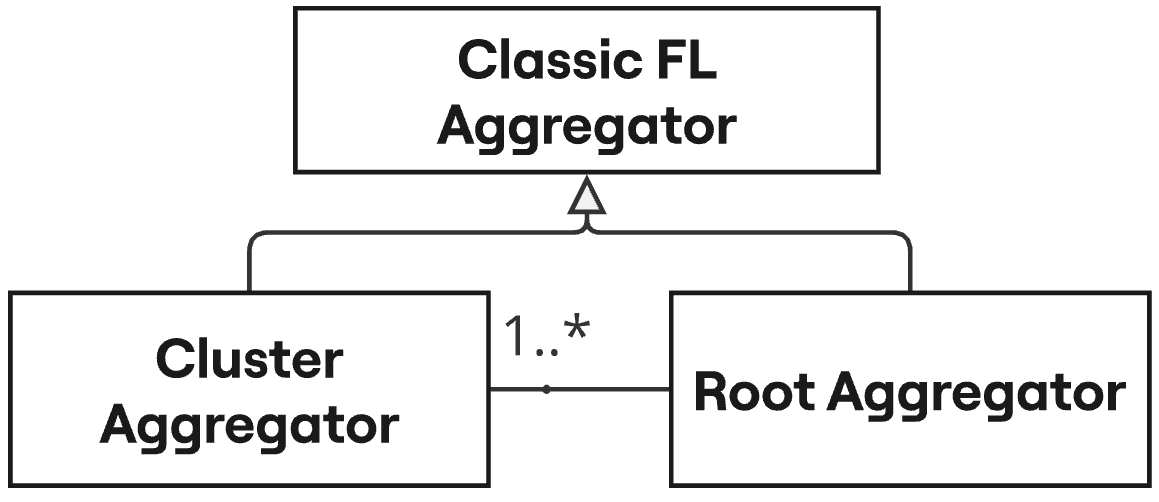
\includegraphics[width=0.55\textwidth]{uml_analysis_object_model_aggregators.png}
    \caption{FLOps Aggregator Types UML Analysis Object Model}
    \label{fig:uml_project_aggregators_analysis_object_model}
\end{figure}

Figure \ref{fig:uml_project_aggregators_analysis_object_model} shows the simplified relation between different FLOps aggregator types.
Because FLOps supports classic and hierarchical FL, it must support different aggregator types.
For conventional FL, FLOps uses the classic aggregators.
For HFL, FLOps creates a single root aggregator and one cluster aggregator per cluster, which are available in the orchestrator.
The root orchestrator sees cluster orchestrators as plain learners.
A cluster aggregator is a hybrid between an aggregator and a learner.